\documentclass{standalone}
\usepackage{tikz}
\usetikzlibrary{patterns, positioning}
\usepackage[sfdefault]{ClearSans} %% option 'sfdefault' activates Clear Sans as the default text font
\usepackage[T1]{fontenc}

\begin{document}
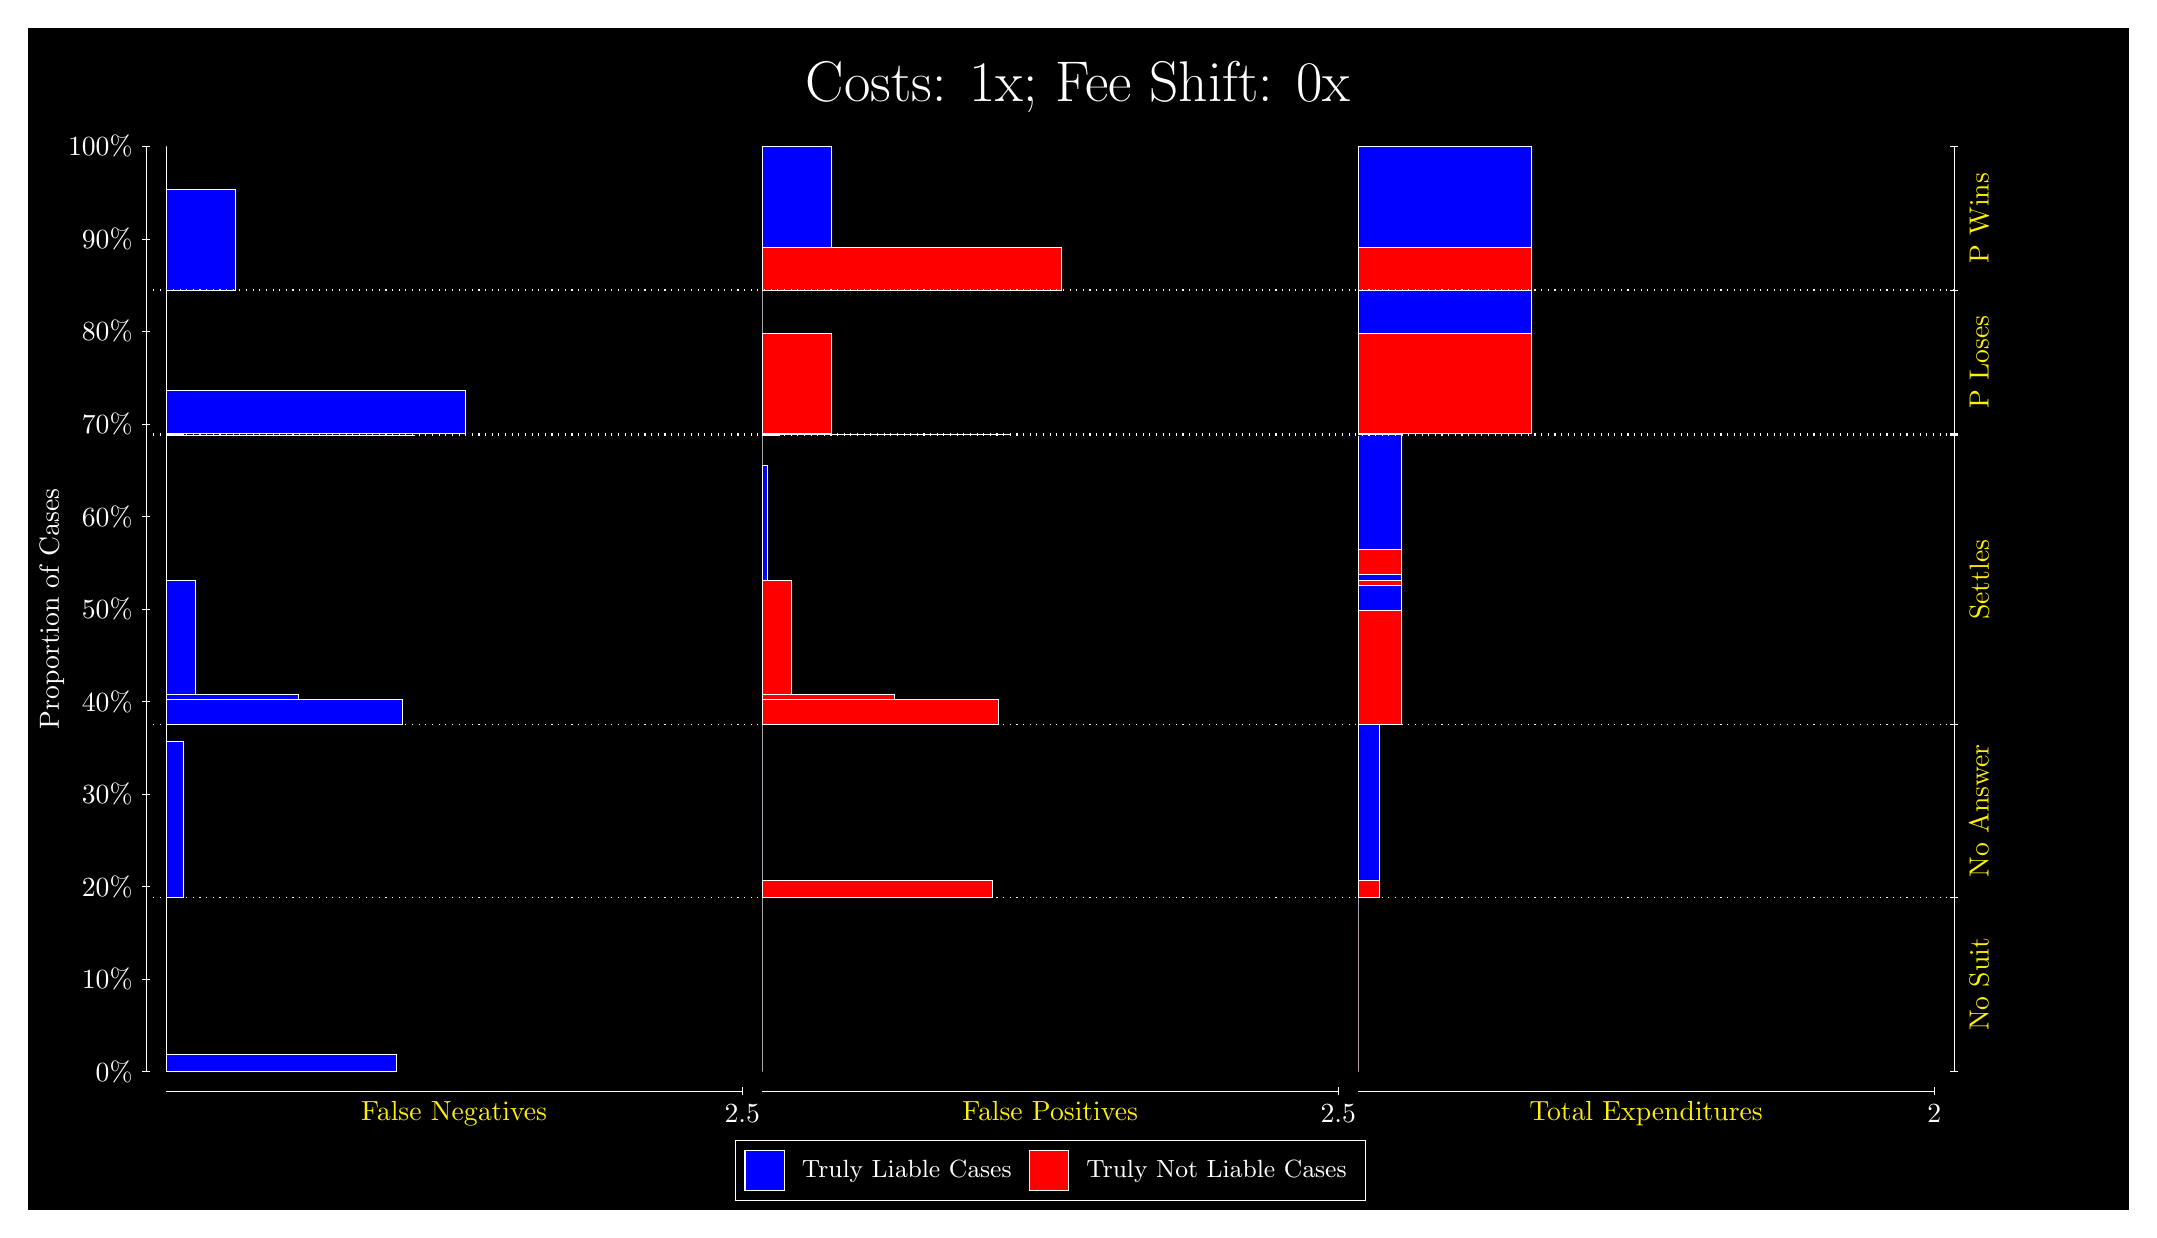
\begin{tikzpicture}
\draw[fill=black] (0,0) rectangle (26.667,15);
\draw[text=white] (0,13.5) rectangle (26.667,15) node[midway] {\huge Costs: 1x; Fee Shift: 0x};
\draw[white, very thin] (1.5,1.75) -- (1.5,13.5);
\node[rotate=90, text=white, anchor=center] at (0.3, 7.625) {Proportion of Cases};
\draw[white, very thin] (1.45,1.75) -- (1.55,1.75);
\node[text=white, anchor=east] at (1.45, 1.75) {0\%};
\draw[white, very thin] (1.45,2.925) -- (1.55,2.925);
\node[text=white, anchor=east] at (1.45, 2.925) {10\%};
\draw[white, very thin] (1.45,4.1) -- (1.55,4.1);
\node[text=white, anchor=east] at (1.45, 4.1) {20\%};
\draw[white, very thin] (1.45,5.275) -- (1.55,5.275);
\node[text=white, anchor=east] at (1.45, 5.275) {30\%};
\draw[white, very thin] (1.45,6.45) -- (1.55,6.45);
\node[text=white, anchor=east] at (1.45, 6.45) {40\%};
\draw[white, very thin] (1.45,7.625) -- (1.55,7.625);
\node[text=white, anchor=east] at (1.45, 7.625) {50\%};
\draw[white, very thin] (1.45,8.8) -- (1.55,8.8);
\node[text=white, anchor=east] at (1.45, 8.8) {60\%};
\draw[white, very thin] (1.45,9.975) -- (1.55,9.975);
\node[text=white, anchor=east] at (1.45, 9.975) {70\%};
\draw[white, very thin] (1.45,11.15) -- (1.55,11.15);
\node[text=white, anchor=east] at (1.45, 11.15) {80\%};
\draw[white, very thin] (1.45,12.325) -- (1.55,12.325);
\node[text=white, anchor=east] at (1.45, 12.325) {90\%};
\draw[white, very thin] (1.45,13.5) -- (1.55,13.5);
\node[text=white, anchor=east] at (1.45, 13.5) {100\%};

\draw[white, very thin] (24.457,1.75) -- (24.457,13.5);
\draw[white, very thin] (24.407,1.75) -- (24.507,1.75);
\node[anchor=west] at (24.407, 1.75) {};
\draw[white, very thin] (24.407,3.9624) -- (24.507,3.9624);
\node[anchor=west] at (24.407, 3.9624) {};
\draw[white, very thin] (24.407,6.159) -- (24.507,6.159);
\node[anchor=west] at (24.407, 6.159) {};
\draw[white, very thin] (24.407,9.831) -- (24.507,9.831);
\node[anchor=west] at (24.407, 9.831) {};
\draw[white, very thin] (24.407,9.8401) -- (24.507,9.8401);
\node[anchor=west] at (24.407, 9.8401) {};
\draw[white, very thin] (24.407,9.8494) -- (24.507,9.8494);
\node[anchor=west] at (24.407, 9.8494) {};
\draw[white, very thin] (24.407,11.675) -- (24.507,11.675);
\node[anchor=west] at (24.407, 11.675) {};
\draw[white, very thin] (24.407,13.5) -- (24.507,13.5);
\node[anchor=west] at (24.407, 13.5) {};

\draw[white, very thin, fill=blue] (1.75,1.75) rectangle (4.6775,1.9721);
\draw[white, very thin, fill=red] (1.75,1.9721) rectangle (1.75,3.9624);
\draw[white, very thin, fill=blue] (1.75,3.9624) rectangle (1.9696,5.9447);
\draw[white, very thin, fill=red] (1.75,5.9447) rectangle (1.75,6.159);
\draw[white, very thin, fill=blue] (1.75,6.159) rectangle (4.7507,6.4717);
\draw[white, very thin, fill=blue] (1.75,6.4717) rectangle (3.4333,6.5407);
\draw[white, very thin, fill=blue] (1.75,6.5407) rectangle (2.1159,7.9949);
\draw[white, very thin, fill=red] (1.75,7.9949) rectangle (1.75,9.831);
\draw[white, very thin, fill=blue] (1.75,9.831) rectangle (4.8971,9.8331);
\draw[white, very thin, fill=red] (1.75,9.8331) rectangle (1.75,9.8401);
\draw[white, very thin, fill=blue] (1.75,9.8401) rectangle (1.9696,9.8474);
\draw[white, very thin, fill=red] (1.75,9.8474) rectangle (1.75,9.8494);
\draw[white, very thin, fill=blue] (1.75,9.8494) rectangle (5.5558,10.399);
\draw[white, very thin, fill=red] (1.75,10.399) rectangle (1.75,11.675);
\draw[white, very thin, fill=blue] (1.75,11.675) rectangle (2.6283,12.951);
\draw[white, very thin, fill=red] (1.75,12.951) rectangle (1.75,13.5);
\draw[white, very thin, fill=red] (9.3189,1.75) rectangle (9.3189,3.7403);
\draw[white, very thin, fill=blue] (9.3189,3.7403) rectangle (9.3189,3.9624);
\draw[white, very thin, fill=red] (9.3189,3.9624) rectangle (12.246,4.1767);
\draw[white, very thin, fill=blue] (9.3189,4.1767) rectangle (9.3189,6.159);
\draw[white, very thin, fill=red] (9.3189,6.159) rectangle (12.32,6.4716);
\draw[white, very thin, fill=red] (9.3189,6.4716) rectangle (11.002,6.5406);
\draw[white, very thin, fill=red] (9.3189,6.5406) rectangle (9.6848,7.9951);
\draw[white, very thin, fill=blue] (9.3189,7.9951) rectangle (9.3921,9.4493);
\draw[white, very thin, fill=blue] (9.3189,9.4493) rectangle (9.3189,9.831);
\draw[white, very thin, fill=red] (9.3189,9.831) rectangle (9.5384,9.8381);
\draw[white, very thin, fill=blue] (9.3189,9.8381) rectangle (9.3189,9.8401);
\draw[white, very thin, fill=red] (9.3189,9.8401) rectangle (12.466,9.8422);
\draw[white, very thin, fill=blue] (9.3189,9.8422) rectangle (9.5384,9.8494);
\draw[white, very thin, fill=red] (9.3189,9.8494) rectangle (10.197,11.126);
\draw[white, very thin, fill=blue] (9.3189,11.126) rectangle (9.3189,11.675);
\draw[white, very thin, fill=red] (9.3189,11.675) rectangle (13.125,12.224);
\draw[white, very thin, fill=blue] (9.3189,12.224) rectangle (10.197,13.5);
\draw[white, very thin, fill=red] (16.888,1.75) rectangle (16.888,3.7403);
\draw[white, very thin, fill=blue] (16.888,3.7403) rectangle (16.888,3.9624);
\draw[white, very thin, fill=red] (16.888,3.9624) rectangle (17.162,4.1767);
\draw[white, very thin, fill=blue] (16.888,4.1767) rectangle (17.162,6.159);
\draw[white, very thin, fill=red] (16.888,6.159) rectangle (17.437,7.6135);
\draw[white, very thin, fill=blue] (16.888,7.6135) rectangle (17.437,7.9262);
\draw[white, very thin, fill=red] (16.888,7.9262) rectangle (17.437,7.9952);
\draw[white, very thin, fill=blue] (16.888,7.9952) rectangle (17.437,8.0643);
\draw[white, very thin, fill=red] (16.888,8.0643) rectangle (17.437,8.3769);
\draw[white, very thin, fill=blue] (16.888,8.3769) rectangle (17.437,9.831);
\draw[white, very thin, fill=red] (16.888,9.831) rectangle (17.437,9.8381);
\draw[white, very thin, fill=blue] (16.888,9.8381) rectangle (17.437,9.8401);
\draw[white, very thin, fill=red] (16.888,9.8401) rectangle (17.437,9.8422);
\draw[white, very thin, fill=blue] (16.888,9.8422) rectangle (17.437,9.8494);
\draw[white, very thin, fill=red] (16.888,9.8494) rectangle (19.083,11.126);
\draw[white, very thin, fill=blue] (16.888,11.126) rectangle (19.083,11.675);
\draw[white, very thin, fill=red] (16.888,11.675) rectangle (19.083,12.224);
\draw[white, very thin, fill=blue] (16.888,12.224) rectangle (19.083,13.5);
\draw[white, dotted] (1.5,3.9624) -- (24.457,3.9624);
\draw[white, dotted] (1.5,6.159) -- (24.457,6.159);
\draw[white, dotted] (1.5,9.831) -- (24.457,9.831);
\draw[white, dotted] (1.5,9.8401) -- (24.457,9.8401);
\draw[white, dotted] (1.5,9.8494) -- (24.457,9.8494);
\draw[white, dotted] (1.5,11.675) -- (24.457,11.675);
\draw[white, very thin] (1.75,1.5) -- (9.0689,1.5);
\node[text=yellow, anchor=north] at (5.4094, 1.5) {False Negatives};
\draw[white, very thin] (9.0689,1.45) -- (9.0689,1.55);
\node[text=white, anchor=north] at (9.0689, 1.45) {2.5};

\draw[white, very thin] (9.3189,1.5) -- (16.638,1.5);
\node[text=yellow, anchor=north] at (12.978, 1.5) {False Positives};
\draw[white, very thin] (16.638,1.45) -- (16.638,1.55);
\node[text=white, anchor=north] at (16.638, 1.45) {2.5};

\draw[white, very thin] (16.888,1.5) -- (24.207,1.5);
\node[text=yellow, anchor=north] at (20.547, 1.5) {Total Expenditures};
\draw[white, very thin] (24.207,1.45) -- (24.207,1.55);
\node[text=white, anchor=north] at (24.207, 1.45) {2};

\node[text=yellow, centered, rotate=90] at (24.777, 2.8562) {No Suit};
\node[text=yellow, centered, rotate=90] at (24.777, 5.0607) {No Answer};
\node[text=yellow, centered, rotate=90] at (24.777, 7.995) {Settles};


\node[text=yellow, centered, rotate=90] at (24.777, 10.762) {P Loses};
\node[text=yellow, centered, rotate=90] at (24.777, 12.587) {P Wins};

\draw (12.978300999999998,1.5) node[draw=none] (baseCoordinate) {};
\begin{scope}[align=center]
        \matrix[scale=0.5, draw=white, below=0.5cm of baseCoordinate, nodes={draw}, column sep=0.1cm]{
            \node[rectangle, draw, minimum width=0.5cm, minimum height=0.5cm, fill=blue] {}; &
            \node[draw=none, font=\small, text=white] (B) {Truly Liable Cases}; &
            \node[rectangle, draw, minimum width=0.5cm, minimum height=0.5cm, fill=red] {}; &
            \node[draw=none, font=\small, text=white] (B) {Truly Not Liable Cases}; \\
            };
\end{scope}

\end{tikzpicture}
\end{document}